\documentclass[12pt]{article}

\usepackage{sbc-template}

\usepackage{graphicx,url}
\usepackage{csvsimple}
\usepackage{subfigure}
\usepackage{algorithm}
\usepackage{algpseudocode}
\usepackage{placeins}
\usepackage{listings}
\usepackage{amssymb}% http://ctan.org/pkg/amssymb
\usepackage{pifont}% http://ctan.org/pkg/pifont
\newcommand{\cmark}{\ding{51}}%
\newcommand{\xmark}{\ding{55}}%
\usepackage{amsmath}
\usepackage{multirow}
\usepackage[brazil]{babel}    
\usepackage[utf8]{inputenc}
 
\sloppy

\title{Simulação de \textit{tracking} da dinâmica dos elétrons em um acelerador
síncrotron}

\author{Gustavo Ciotto Pinton\inst{1} - RA117136 }


\address{Instituto de Computação -- Universidade Estadual de Campinas
(UNICAMP)\\
  Av. Albert Einstein, 1251, Cidade Universitária, Campinas/SP \\
  Brasil, CEP 13083-852, Fone: [19] 3521-5838
  \email{gustavociotto@gmail.com}
}

\begin{document} 

\maketitle

\begin{abstract}
This report presents and describes the main aspects of the development of a
parallel solution for a sequential algorithm, whose purpose is simulating
the dynamics (modeled by a 6-element vector \(X\)) of electrons that
run through a synchrotron accelerator. In general, in this algorithm, the whole
extension of the accelerator is divided into several elements capable of
changing the state of each electron in a certain way, and it is sought to
determine which initial conditions of \(X\) will meet some conditions after a
certain number of revolutions. All the parallelization was based on GPUs and the
CUDA library, obtaining gains of performance of the order of 2500\% compared
to the serial execution.
\end{abstract}
     
\begin{resumo} 
Este relatório apresenta e descreve os principais aspectos do
desenvolvimento de uma solução paralela para um algoritmo sequencial de
simulação da dinâmica do movimento dos elétrons (modelado por um vetor \(X\) de
6 posições) que percorrem um acelerador síncrotron. De maneira geral, neste
algoritmo, divide-se toda a extensão do acelerador em diversos elementos capazes de alterar o estado de cada életron de
uma determinada maneira, e busca-se quais condições iniciais de \(X\) atenderão
algumas condições após um determinado número de voltas. Toda a paralelização foi
baseada em GPUs e na biblioteca CUDA, obtendo-se ganhos de performance da ordem
de 2500\% em relação à execução serial.
\end{resumo}


\section{Introdução}

Aceleradores de partículas síncrotron são constituídos, ao longo de todas suas
circunferências, de atuadores, tais como dipolos, quadrupólos e sextupólos,
responsáveis por modificar a direção dos elétrons através da imposição de campos
magnéticos. Pode-se modelar o estado de um elétron na entrada do acelerador por
um vetor no espaço de fase constituído por 6 elementos \( X = (x_1, x_2, \ldots,
x_6) \). A cada passagem por um determinado atuador, esse vetor é modificado por
um mapa \(F_n(X)\) que depende, evidentemente, do tipo de atuador e de seus
parâmetros. A simulação de \textit{tracking} da dinâmica de movimento dos
elétrons consiste, portanto, em determinar quais vetores iniciais \(X_i\) neste
espaço de fase correspondem à órbitas estáveis após o percurso de \(N\) voltas
pelo acelerador. Um vetor \(X_i\) pode ser considerado uma
órbita estável somente se, ao fim de \(N\) voltas completas, as posições \(x_1,
\ldots, x_6 \) são inferiores às constantes \(C_1, \ldots, C_6\). A explicação
dos significados físicos de cada uma dessas posições não faz parte do escopo
deste artigo.

Durante os experimentos, o acelerador foi modelado por um número
constante \(M = 10000\) de atuadores e a cardinalidade do conjunto de vetores
iniciais testados foi igual a \(I = 10000\). Além disso, variou-se o número de
voltas \(N\) entre 10 e 10000, de modo a avaliar o ganho de performance em
função do número total de iterações desenvolvidas.

Aproveitando-se a alta densidade de \textit{cores} de arquitetura SIMD
encontrada nas GPUs atuais, a paralelização desta simulação consistiu em
distribuir o cálculo de cada condição inicial \(X_i\) em uma \textit{thread}
distinta executada pela GPU, de modo a maximizar a quantidade de
\textit{threads} que rodam simultaneamente. A implementação foi a baseada no
\textit{toolkit CUDA}, desenvolvido para as placas de vídeo da \textit{NVIDIA}.
Como todos os vetores \(X_i\) passarão pelos mesmos atuadores na mesma ordem e
não farão acessos a posições não sequenciais de memória, a paralelização deste
algoritmo não foi afetado pelos principais fatores que degradam a performance
neste tipo de arquitetura, sendo eles, respectivamente, \textit{branching
divergence} e acessos \textit{non-coalesced} à memória.

As próximas seções são dedicadas aos processos de implementação e aos resultados
obtidos.

\section {Análise da execução sequencial}

Com o intuito de identificar qual trecho do programa possui o maior potencial de
paralelização, a ferramenta \texttt{gprof} foi utilizada. Esse aplicativo é
capaz de calcular o tempo de execução gasto para cada função, permitindo, assim,
ao desenvolvedor uma visão global do desempenho do seu programa. Em
essência, duas análises sõa oferecidas por ele, sendo elas, a \textit {flat
profile} e a \textit{call graph}. A primeira mostra quanto tempo o programa
gastou em cada função e quantas vezes tal função foi chamada. A segunda, por sua
vez, permite, para cada função, visualizar quais outras funções ela chamou
e por quais outras funções ela foi chamada. Essa análise pode ser útil para a
determinação de trechos em que chamadas que tomam muito tempo podem ser
economizadas.

A tabela \ref{tab:flat} abaixo corresponde à fração mais relevante da análise
\textit{flat profile}, obtida através da execução da versão sequencial da
simulação com \(N = 10\). 

\begin{table}[h]
    \centering
    \small
	\caption{\label{tab:flat} Análise \textit{flat profile} da execução sequencial.}
	\begin{tabular}{| p{0.09\textwidth} | p{0.1\textwidth} | p{0.1\textwidth} |
	p{0.125\textwidth} | c | }
		\hline
		\textbf{\% time} & \textbf{cumul. seconds} & \textbf{self seconds} &
		\textbf{calls} & \textbf{name} \\ \hline 
		28.87 & 2.27 & 2.27  & 100000  & DynamicSearch::\textbf{performOneTurn(double (\&))} \\\hline 
		15.77 & 3.51 & 1.24  & 1200000020 & std::vector\(<\)RingElement\(>\)::\textbf{size()} const \\\hline 
		15.58 & 4.74 & 1.23  & 400000000  & Drift::\textbf{pass(double (\&))} \\\hline
		14.12 & 5.85 & 1.11  & 400000000  & Quadrupole::\textbf{pass(double (\&)} \\\hline
		11.64 & 6.77 & 0.92  & 200000000  & Sextupole::\textbf{pass(double (\&)} \\\hline
		11.45 & 7.67 & 0.90  & 100000000  & std::vector::\textbf{operator[]}(unsigned
		long) \\\hline \ldots & & & & \\\hline
	\end{tabular}
\end{table}

Observa-se, por meio dela, que 97.43\% de todo o tempo
gasto pelo programa está concentrado em apenas 6 funções. A análise do corpo da
função \texttt{dynamical\_aperture\_search()} (contido no arquivo
\texttt{DynamicSearch.cpp}) explica perfeitamente a afirmação anterior, à medida
que explicita três \textit{loops} encadeados. Os dois primeiros são responsáveis
por iterar sobre o conjunto de condições iniciais (de cardinalidade \(I\)),
enquanto que o segundo, por submeter cada uma das condições iniciais a \(N\)
voltas pelos atuadores. A cada iteração do laço mais interior, realiza-se uma
chamada à função \texttt{performOneTurn(double *)}, que, por sua vez, chama o
método \texttt{pass} de cada um dos \(M\) atuadores.
Desta forma, em linhas gerais, \(I * N * M\) iterações serão executadas apenas
neste trecho de código. É importante ressaltar que os dois \textit{loops}
responsáveis pela iteração sobre as condições iniciais podem ser classificados
como \textit{doall loops} e, portanto, podem ser paralelizados. Isso porque o
processo de iteração de uma condição inicial \(X_{i1}\) é
totalmente independente do processo associado à condição
\(X_{i2}\). Em oposição, o laço mais interior e aquele presente na função
\texttt{performOneTurn} são classificados como \textit{doacross loops}, visto
que as iterações executadas por eles dependem obrigatoriamente de resultados
gerados por iterações anteriores. Essa afirmação é facilmente verificada em
ambos os casos: para que a volta de índice \(i\) seja executada, ela
necessita dos resultados que as de índices \(i - 1, i - 2, \ldots, 0\)
produziram, e para que o estado do életron seja calculado no atuador \(M_i\), é
necessário que os estados associados aos atuadores \(M_{i-1}, M_{i-2},\ldots,
M_{0}\) sejam conhecidos.

% \begin{table}[h]
%     \centering
%     \small
% 	\caption{\label{tab:call} Análise \textit{call graph} da execução sequencial.}
% 	\begin{tabular}{| p{0.09\textwidth} | p{0.1\textwidth} | p{0.10\textwidth} | l | }
% 		\hline
% 		\textbf{\% time} & \textbf{self seconds} & \textbf{children}  & \textbf{name} \\ \hline 
% 		 & 2.27 & 5.39 & \textbf{DefaultDynamicSearch::dynamical\_aperture\_search()} \\\hline
% 		 \textbf{97.3} & 2.27 & 5.39 & DynamicSearch::\textbf{performOneTurn(double (\&))} \\\hline
% 		 & 1.24 & 0 & std::vector::operator[](unsigned long) \\\hline
% 		 & 1.24 & 0 & std::vector::operator[](unsigned long) \\\hline
% 		 & 1.23 & 0 & Drift::\textbf{pass(double (\&))} \\\hline
% 		 & 1.11 & 0 & Quadrupole::\textbf{pass(double (\&)} \\\hline
% 		 & 0.92 & 0 & Sextupole::\textbf{pass(double (\&)} \\\hline
% 		 \ldots & & & \\\hline
% 	\end{tabular}
% \end{table}

\section {Paralelização}

Esta seção é dedicada ao detalhamento do processo de implementação de um
algoritmo paralelo baseado em CUDA e das principais dificuldades encontradas e
como elas foram resolvidas.

\subsection{Implementação}

A fim de paralelizar a execução dos \textit{doall loops} detectados na seção
anterior, distribui-se a computação de cada condição inicial em uma
\textit{thread} distinta. Como discutido nesta mesma seção, isso pode ser
realizado dado que tais cálculos são completamente independentes entre si.

CUDA distribui as \textit{threads} em blocos unidimensionais, bidimensionais ou
tridimensionais de até 1024 \textit{threads}. Essa limitação existe devido ao
fato de que todas as \textit{threads} de um mesmo bloco residem no mesmo
\textit{core} e, desta forma, compartilham memória e tempo de processamento
\cite{cuda}. A multidimensionalidade dos blocos garante que as \textit{threads}
sejam identificadas mais facilmente de acordo com a sua aplicação. No nosso
caso, por exemplo, como as condições inicias são determinadas a partir de uma
tupla \((i,j)\), utilizamos blocos de duas dimensões. Adicionalmente, tendo em
vista que a quantidade máxima de \textit{threads} por bloco é 1024, adota-se,
neste artigo, blocos de \(32\times32\). Assim como as \textit{threads}, blocos
também são distribuídos em \textit{grids} de uma, duas ou três dimensões. Tendo
em vista que a motivação para este tipo de divisão é a mesma que a explicada
anteriormente, utilizaremos também \textit{grids} bidimensionais com dimensões
\(\frac{I_x}{32}\times\frac{I_y}{32}\), em que \(I_x\) e \(I_y\) representam as
dimensões do conjunto de condições iniciais.

\textit{Threads} são executadas simultaneamente em blocos de 32, denominados
\textit{warps}. Tais blocos rodam em uma arquitetura SIMD, isto é, uma única
instrução é capaz de realizar a mesma operação para todas as suas
\textit{threads}. \textit{Warps} são executadas paralelamente por
\textit{streaming multiprocessors}, ou simplesmente \textit{SMs}, cuja
capacidade depende da \textit{compute capability} da GPU. A escolha do número de
\textit{threads} por bloco também deve ser influenciada por essa capacidade, já
que deseja-se maximizar o uso de um \textit{SM}. Para a GPU \textit{NVIDIA Tesla
K40c}, de \textit{compute capability} 3.5 e que foi utilizada nos testes, o
número máximo de \textit{warps} por \textit{SM} é 64, totalizando, desta forma,
2048 \textit{threads} que podem ser executadas simultaneamente \cite{compute}. A
escolha de blocos de 1024 \textit{threads} maxima, portanto, o uso de um
\textit{SM}, à medida que 2 blocos podem ser rodados paralelamente, ocupando,
assim, toda a capacidade do respectivo \textit{SM}.

Com a divisão de \textit{threads} em blocos e \textit{warps} já definida, a
próxima etapa é implementar o \textit{kernel} que será executado em cada uma
delas e que calculará, a partir de uma condição inicial \(X_i\), o respectivo
vetor \(X_f\) após \(N\) voltas por \(M\)
atuadores. Tal função recebe como parâmetro, além de \(N\) e \(M\), o vetor
\(A\) de \texttt{struct} contendo os atributos que descrevem cada um dos \(M\)
atuadores. É importante ressaltar que, inicialmente, a ideia era transmitir um
vetor de objetos que herdassem da classe abstrata \texttt{DynamicSearch} e que
possuíssem as suas próprias implementações dos métodos virtuais. Porém, conforme
discutido na subseção \textbf{Dificuldades}, esse tipo de operação não é
suportado por \textit{CUDA}. Adicionalmente, o \textit{kernel} recebe também
como paramêtro o vetor $R$, cujo propósito é armazenar os resultados calculados
por todas as \textit{threads}, de maneira que eles possam ser copiados para a
memória da CPU posteriormente. Enfim, como a condição inicial depende dos
índices \((i,j)\) da \textit{thread} em que ela será utilizada, ela pode ser
calculada internamente e não necessita, portanto, ser transmitida ao
\textit{kernel} através de parâmetros. O pseudo-código \ref{alg:cuda}, a seguir,
exemplica as operações desenvolvidas por cada \textit{thread} na GPU.


\begin{algorithm}
\caption{\label{alg:cuda} \textit{Pseudo-código} do \textit{kernel} que é
executado pela GPU} \begin{algorithmic}[1]
  \Function{dynamicSearchKernel}{$A,M,N,R$}
  	\State ${i} \gets \text{blockDim.y} * \text{blockIdx.y} + \text{threadIdx.y} $ \Comment{Índice y da \textit{thread}} 
  	\State ${j} \gets \text{blockDim.x} * \text{blockIdx.x} + \text{threadIdx.x} $ \Comment{Índice x da \textit{thread}}  
    \State ${X_i} \gets f(i,j) $ \Comment{Calcula condição inicial \(X_i\) em função de \(i\) e \(j\)}
    \For{$n \gets 0$ to ${N}$} \Comment{Itera sobre o número de voltas}
        \For{$m \gets 0$ to ${M}$} \Comment{Itera sobre o número de atuadores}
        	\State $X_i \gets g_{A[m]} (X_i)$ \Comment{Altera \(X_i\) de acordo com atuador \(A[m]\)}
    	\EndFor
    \EndFor
    \State ${R[i,j]} \gets X_i $ \Comment{Armazena resultado calculado}
   \EndFunction

\end{algorithmic}
\end{algorithm}

Vale lembrar que \(A\) e \(R\) devem ser alocados na memória do dispositivo
através da chamada da função \texttt{cudaMalloc} e seus respectivos conteúdos
devem ser copiados de/para a GPU através de \texttt{cudaMemCpy}. Ao fim, as
memórias alocados são liberadas novamente por meio da função \texttt{memFree}.

\subsection{Dificuldades}

Duas principais dificuldades foram encontradas no desenvolvimento da solução
paralela. Elas serão abordadas nas próximas subseções.

\subsubsection{Objetos com métodos virtuais}

Uma das principais classes que compõem o algoritmo sequencial é a classe
abstrata \texttt{RingElement}, cujo principal propósito é fornecer uma base para
a implementação de objetos capazes de representar um atuador. Na nossa
aplicação, por exemplo, são fornecidas três classes que herdam diretamente de
\texttt{RingElement}: \texttt{Drift}, \texttt{Quadrupole} e \texttt{Sextupole}.
Tais classes fornecem uma implementação ao método virtual \texttt{pass()},
dependendo, evidentemente, de como influenciam na dinâmica de um elétron. O
principal objetivo buscado ao empregar esse modelo de implementação é fornecer
uma maneira simples e rápida para a adição de diferentes atuadores.

Assim como na solução sequencial, buscou-se utilizar essa abstração também na
implementação de um \textit{kernel} capaz de ser executado na GPU. A princípio,
portanto, tal \textit{kernel} receberia, como parâmetro, um vetor de objetos
cujas classes herdassem de \texttt{RingElement} e, internamente, chamaria os
métodos \texttt{pass()} corretamente de acordo com a classe derivada de cada
elemento do vetor. Entretanto, a concretização desta proposta não foi possível, graças a uma
limitação presente em \textit{CUDA}. Segundo \cite{virtual}, não é permitido
transmitir um objeto de uma classe com métodos virtuais como parâmetro a uma
função \texttt{\_\_global\_\_}. Isso porque, de acordo com este mesmo documento,
a tabela de funções virtuais é colocada em uma posição de memória constante
ou global pelo compilador \texttt{nvcc} e, desta forma, é inacessível
internamente ao dispositivo.

A solução empregada a fim de contornar esse problema foi utilizar uma
\texttt{struct} contendo todos os atributos de todas as classes derivadas de
\texttt{RingElement}. Apesar do fato de que esta solução não otimiza o consumo
de memória da GPU, sua simplicidade torna a adição de novos atuadores próxima da
maneira original da solução sequencial.

\subsubsection{Divergência das operações em ponto flutuante}

Após que os primeiros resultados da solução paralela foram obtidos, sua
comparação com aqueles da aplicação sequencial revelou que apenas um subconjunto
bem reduzido dos vetores finais \(X_f\) divergia e, na maioria das vezes, essa
divergência era encontrada a partir da terceira ou quarta casas decimais. Para
\(N = 10\) voltas, \(M = 10000\) atuadores e um conjunto de entrada de
cardinalidade \(I = 10000\), por exemplo, dentre os 6100 vetores \(X_f\)
encontrados pelas duas soluções, apenas um dentre eles divergia. A tabela
\ref{tab:div}, abaixo, exemplifica este caso. Para a compilação do programa
sequencial, foi utilizada explicitamente a \textit{flag} \texttt{-msse2},
instruindo o compilador a empregar a extensão SSE para o cálculo das operações
em ponto flutuante.

\begin{table}[h]
    \centering
    \small
	\caption{\label{tab:div} Vetores \(X_f\) divergentes entre as execuções
	paralela e sequencial.}
	\begin{tabular}{| c | c | c | c | c | c | c | }
		\hline
		 & \(X_f[0]\) & \(X_f[1]\) & \(X_f[2]\) & \(X_f[3]\) & \(X_f[4]\) & \(X_f[5]\) \\ \hline 
		Serial & 0.021950 & 0.000676  & 0.000370  & 0.000091 & 0.0 & 0.0 \\\hline 
		CUDA & 0.022004 & 0.000684  & -0.001117  & -0.000063 & 0.0 & 0.0 \\\hline 
	\end{tabular}
\end{table}

Uma depuração profunda do código eliminou a primeira hipótese de que o
\textit{kernel} escrito não era compatível com a versão \textit{serial}. A
segunda hipótese, posteriormente confirmada, foi de que as pequenas variações
observadas vinham do fato de que as operações de ponto flutuante fossem
realizadas de maneira distinta entre a CPU e a GPU. Uma análise de
\cite{ieee754} determinou que, de fato, diferenças poderiam ser encontradas em
relação ao conjunto de instruções SSE, utilizado pela CPU para este tipo de
cálculo no exemplo acima. Segundo este artigo, GPUs com \textit{compute
capability} \(\ge2.0\), como a que foi utilizada nos testes, suportam um tipo de
operação denominada \textit{fused-multiply-add} (ou simplesmente \textit{FMA})
em pontos flutuantes de precisão simples e dupla, cujo principal objetivo é
executar uma multiplicação e uma adição, isto é, computar \(X * Y + Z\), através
de uma única instrução. Sua principal vantagem, além do ganho em performance por
executar duas operações de uma única vez, é que ela realiza um arredondamento a
menos que uma operação de multiplicação seguida por uma de adição. Desta forma,
denotando-se um arredondamento por \(rn(x)\), o resultado de uma instrução
\textit{FMA} seria \(rn(X*Y+Z)\), enquanto que o resultado de duas instruções,
\(rn(rn(X*Y) + Z)\). Evidentemente, a precisão após dois arrendodamentos é
inferior a um apenas. Ao contrário do que ocorre no \texttt{nvcc}, a operação
\textit{FMA} não é habilitada por padrão no compilador \texttt{gcc} e o seu uso
requer uma indicação explícita por meio de funções e \textit{flags} específicas.
Tal discordância foi justamente a fonte da divergência observada em uma pequena
parte das soluções. Outra evidência constatada durante os testes e que confirma
essa afirmação baseia-se no fato de que para \(N\) superiores, a quantidade de
vetores \(X_f\) é superior. Isso significa que as diferenças geradas nos
cálculos intermediários são propagadas e, quanto maior for o valor de \(N\),
mais elas serão potencializadas pelas iterações seguintes.

Os autores de \cite{ieee754} afirmam que, para desabilitar o uso de instruções
\textit{FMA} na GPU, é necessário utilizar funções intrínsicas que informem ao
compilador explicitamente para não unir uma multiplicação e uma adição. Neste
caso, \(X*Y + Z\) seria transformada na sentença
\texttt{\_\_dadd\_rn(\_\_dmul\_rn(X,Y), Z)}. Aplicando-se este
mesmo princípio à nossa aplicação,  a fim de obtermos os mesmos resultados
que a execução sequencial, foi necessário o uso destas funções em todas as
sentenças que realizavam algum tipo de operação aritmética, mantendo,
inclusive, a ordem dos operandos. Desta forma, a sentença \texttt{r[0] +=
length * r[1]} seria representada em CUDA por \path{__dadd_rn(r[0],
__dmul_rn(length, r[1]))}, por exemplo. Em adição, o uso de instruções
\textit{FMA} também pode ser desabilitado através da \textit{flag}
\texttt{--fmad} do compilador \texttt{nvcc}. Caso ela seja modificada para 0 ou
\textit{false}, o compilador não gerará instruções que utilizem essa
\textit{feature}.

É importante ressaltar que nenhuma das duas soluções apresentadas acima está
mais certa ou mais errada do que a outra. De fato, elas tratam-se apenas de
tentativas de se aproximar de um valor cuja representação não pode ser fielmente
realizada por meio de 32 ou 64 \textit{bits}.

\section{Resultados}

Os resultados apresentados nesta seção foram gerados em um servidor com um
processador \textit{Intel(R) Xeon(R) E5-2620 v4} e com uma GPU \textit{NVIDIA
Tesla K40c} com \textit{compute capability} 3.5. O código sequencial foi
compilado com o compilador \texttt{gcc} com as \textit{flags} \texttt{-O3},
\texttt{-Wall}, \texttt{--std=c++11}, \texttt{-mfpmath=sse} e
\texttt{-sse2}. As duas últimas garantem que a extensão SSE será utilizada e que
as operações em ponto flutuante sigam o padrão IEEE 754, tanto para precisão
simples quanto para a dupla, assim como o compilador CUDA \texttt{nvcc} garante
\cite{ieee754}. Essas \textit{flags} impedem que outras extensões sejam
utilizadas, tais como a x87, que emprega precisão dupla-extendida com
registradores de 80 \textit{bits} com 64 deles dedicados somente à mantissa.
\cite{monniaux:hal-00128124}. Operações realizadas nestes registradores
produziriam resultados mais precisos, mas incompatíveis com os geradores com
precisão dupla, que seguem estritamente o padrão IEEE 754.

Duas implementações paralelas foram realizadas, uma com suporte a instruções
\textit{FMA} e a outra compatível com a aplicação sequencial compilada conforme
descrito acima. Para tal, foram propostas duas constantes, \texttt{CUDA\_FMA}
e \texttt{CUDA\_INTRINSICS}, uma para cada implementação respectivamente. A
escolha de qual delas deve ser utilizada é feita por meio da \textit{flag}
\texttt{-D} no comando de compilação.

A imagem \ref{fig:time} resume os resultados encontrados para
as três execuções descritas acima com \(I = 10000\), \(M = 10000\) e quatro
valores distintos de \(N\), sendo eles 10, 100, 1000 e 10000. Verifica-se que 
o tempo de execução cresce proporcionalmente com o número de iterações, isto é,
se o último cresce 10 vez, o outro também aumentará nesta mesma proporção. A
figura \ref{fig:speedup}, por sua vez, contém os \textit{speedups} para cada uma
das execuções. Em média, a solução que utiliza \textit{FMA} tem um
\textit{speedup} de \textbf{26.821}, enquanto que a tradicional, \textbf{20.622}.

\begin{figure}
  \centering
  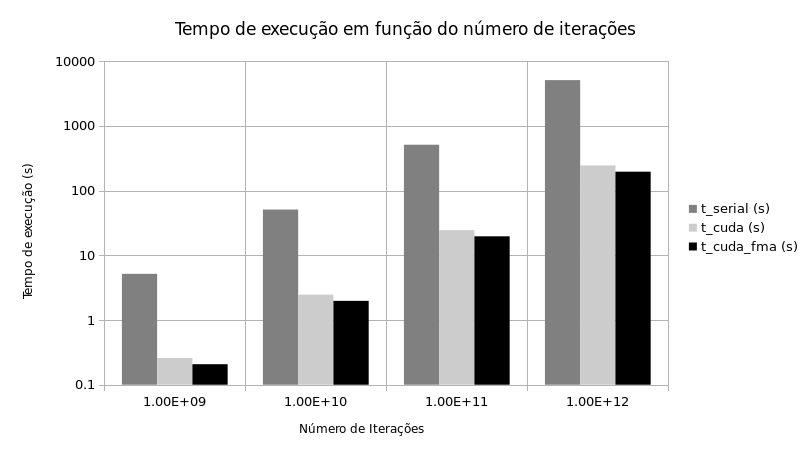
\includegraphics[width=0.9\linewidth]{img/time}
  \caption{Tempos de execução para diversos valores de \(N\)}
  \label{fig:time}
\end{figure}

\begin{figure}
  \centering
  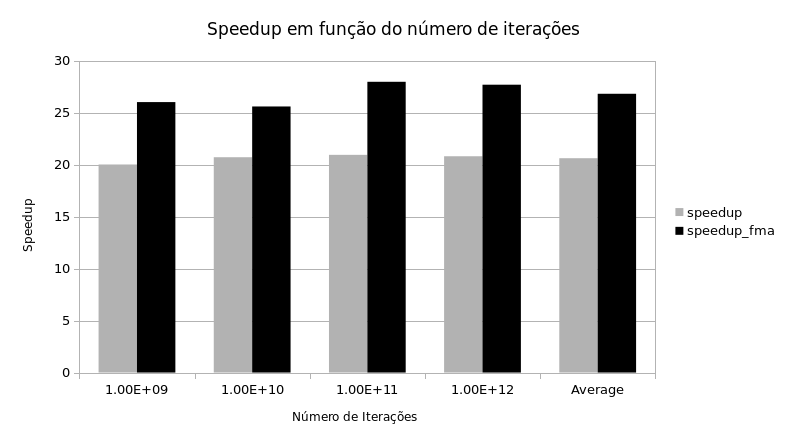
\includegraphics[width=0.9\linewidth]{img/speedup}
  \caption{\textit{Speedup} para diversos valores de \(N\)}
  \label{fig:speedup}
\end{figure}

Observa-se que a melhor performance foi obtida empregando-se instruções
\textit{FMA} em CUDA. Conforme descrito na seção \textbf{Dificuldades}, além de
uma melhor precisão, essa técnica também garante melhor desempenho, à medida que
uma operação de multiplicação e outra de adição são realizadas por uma única
instrução. Em oposição, ela não oferece exatamente os mesmos resultados que a
simulação \textit{serial}, dado o fato que ela realiza apenas um arredondamento
a cada instrução \textit{FMA}, ao contrário da solução tradicional, que produz
dois arrendomentos para esta mesma operação.

\section{Conclusões}

Discutimos e avaliamos as principais dificuldades na paralelização, baseada em
GPUs e CUDA, de um algoritmo de \textit{tracking} da dinâmica de életrons
submetidos em um acelerador síncrotron, . Dentre as principais
dificuldades, destacamos a impossibilidade de transmitir a funções
\path{__global__} objetos com métodos virtuais como parâmetro \cite{virtual} e
as divergências de resultados entre CPU e GPU causadas por maneiras distintas de
se efetuar operações de pontos flutuantes. Propomos, ainda, duas implementações
para o algoritmo sequencial: uma que utilizasse instruções
\textit{fused-multiply-add} capazes de realizar a operação \(X*Y + Z\) de
\textit{uma única vez} e a outra, semelhante ao método tradicional, isto é, que
utizasse duas instruções separadas para esta mesma operação. Para a primeira,
encontrados um \textit{speedup} médio de \textbf{26.821} e, para a segunda,
\textbf{20.622}.

\bibliographystyle{sbc}
\bibliography{sbc-template}

\end{document}
